\chapter{The Standard Model}
The Standard Model of particle physics is a universally accepted framework which explains the interactions of fundamental particles. All known fundamental particles, outlined in Figure \ref{fig:sm}, are represented in the Standard Model. The model describes three of the four known forces: the electromagnetic force, the weak force, and the strong force. Gravity, the fourth fundamental force, is not addressed by the Standard Model. The Standard Model was primarily developed over the course of the 1960s and 1970s, by combining the work of many physicists into one coherent model. The Standard Model has been established as a well-tested theory by decades of experimental physics research.\par

This chapter will seek to introduce the phenomenology and mathematical foundations of the Standard Model, and present the supporting experimental evidence. Phenomenon which are unexplained by the Standard Model such as gravity will be considered at the end of the chapter, leading to an exploration of theories beyond the Standard Model in the subsequent chapter.

\section{Phenomenology: Particles and Forces}
\subsection{Particles}
A classic representation of the particles comprising the Standard Model is shown in Figure \ref{fig:sm}. The two primary particles classes are bosons (gauge bosons and the scalar Higgs boson) and fermions (leptons and quarks). The bosons are carriers of fundamental forces, while the fermions are the building blocks of matter. Fermions are sorted into three \textit{generations}, and each fermion is identified by a unique \textit{flavor}.

\begin{figure}
        \centering
	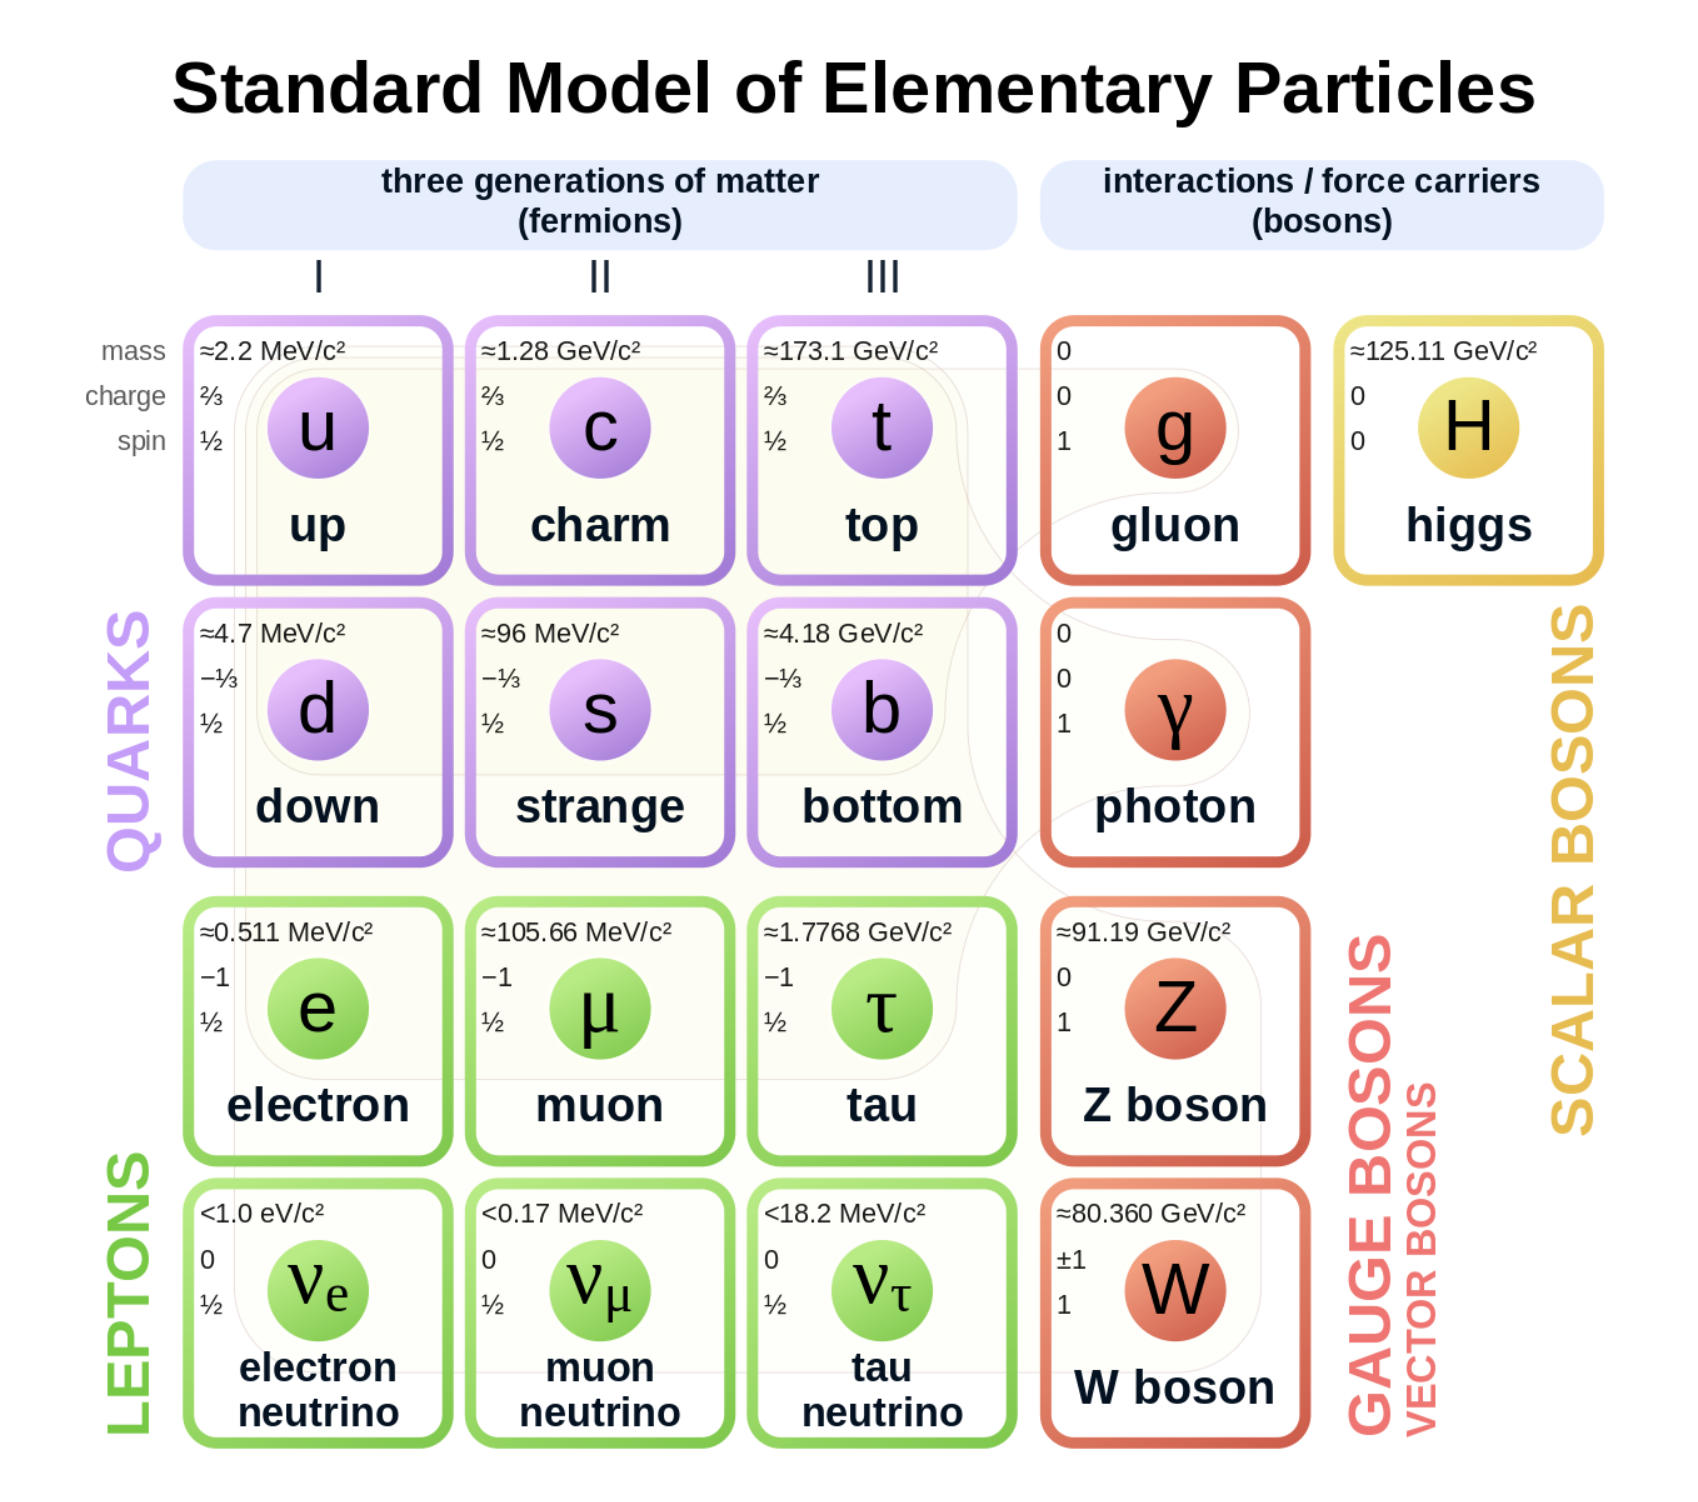
\includegraphics[width=0.8\textwidth]{figures/ch1/standard_model.png}
	\caption{Diagram of the 17 particles comprising the Standard Model}
	\label{fig:sm}
\end{figure}

Each entry in the table in Figure \ref{fig:sm} is accompanied by 3 characteristic numbers: mass, charge, and spin. The mass of each particle is determined to limited precision by experimental observation, with the exception of photons and gluons which are known to be massless. Charge refers to the electromagnetic charge, which is integer for leptons and fractional for quarks. Spin is an intrinsic form of angular momentum carried by fundamental particles; all fermions have half integer spin, while bosons have integer spin. \par

Each particle is also known to have an \textit{antiparticle}. Each antiparticle has the same mass but the opposite charge of their Standard Model counter part; for example, the antiparticle of the electron is the positron, which has all the same properties but a positive charge. The photon, Z boson, and Higgs are each their own antiparticle. The nature of antineutrinos is an open question driving neutrino physics research, as it is not currently known whether neutrinos are their own antiparticle. \par

\subsection{Forces}
The three fundamental forces explained by the Standard Model are the electromagnetic force, the strong force, and the weak force. The photon is the carrier of the electromagnetic force, which dictates the nature of interactions between electrically charged particles, and is widely covered by introductory physics courses. The electromagnetic force has an infinite interaction range, a result of the massless and non-self interaction nature of the photon. The electromagnetic interaction is described by the theory of quantum electrodynamics (QED).\par

The weak force gives rise to atomic radiation and decay. It allows for the processes of beta decay, which enables conversion between neutrons and protons within the nucleus of an atom. In the process of beta decay, a proton decays into a neutron, a positron, and a neutrino; or, a neutron decays into a proton, an electron and an antineutrino. The weak interaction allows for quark flavor mixing, the which enables beta decay. The W\textsuperscript{+}, W\textsuperscript{-}, and Z\textsuperscript{0} are the force carriers of the weak force. The effective range of the weak force is limited to subatomic distances, as a result of the massive nature of the mediator bosons. The unified theory of the electroweak interaction posits that at high enough energies the electromagnetic interaction and the weak force merge into the same force. This threshold is termed the unification energy and calculated to be about 246 GeV \cite{vev}. \par

The strong force confines quarks into hadron particles, such as protons and neutrons. The strong force also allows for the creation of atomic nuclei by binding protons and neutrons together, and is generally referred to as the ``nuclear force" in this context. The gluon is the mediator of the strong force, which is a short-range force which acts at subatomic distances on the order of $10^{-15}$ m. At this range, the strong force is about 100x as strong as the electromagnetic force, which allows for the creation of positively charged nuclei \cite{griffiths}. The strong force is described by the theory of quantum chromodynamics (QCD). In the same way that QED dictates the interaction of electrically charges particles, QCD dictates the interactions of \textit{color-charged} particles. Due to the particular importance of QCD in this thesis, this topic will be explored in detail in section \ref{sec:QCD}. \par

The fundamental Feynmann diagram for each of the three forces discussed here is depicted in Figure \ref{fig:force_feynmann}. The fourth fundamental force, gravity, is not currently explained by any known mechanism within the Standard Model. 

 \begin{figure}
     \centering
     \begin{subfigure}[b]{0.43\textwidth}
         \centering
         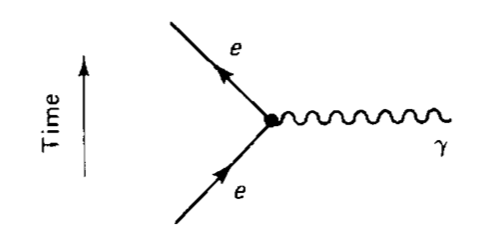
\includegraphics[width=\textwidth]{figures/ch1/em_force.png}
         \caption{The electromagnetic force}
     \end{subfigure}
     \hfill  
     \begin{subfigure}[b]{0.4\textwidth}
         \centering
         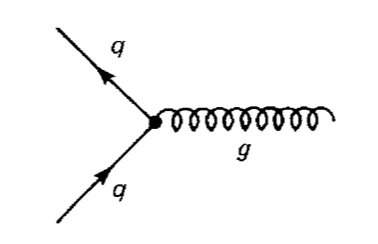
\includegraphics[width=\textwidth]{figures/ch1/strong_force.png}
         \caption{The strong force}
     \end{subfigure} \\
     \hfill
     \begin{subfigure}[b]{0.4\textwidth}
         \centering
         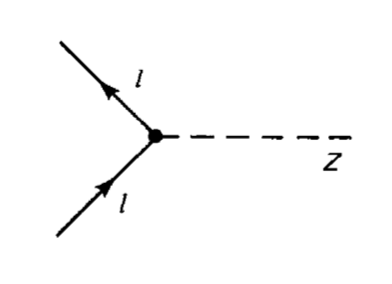
\includegraphics[width=\textwidth]{figures/ch1/weak_neutral.png}
         \caption{The neutral weak force}
     \end{subfigure}
     \hfill  
     \begin{subfigure}[b]{0.4\textwidth}
         \centering
         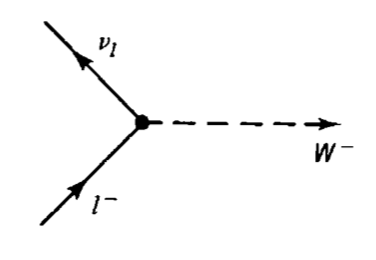
\includegraphics[width=\textwidth]{figures/ch1/weak_charged.png}
         \caption{The charged weak force}
     \end{subfigure} 
     \caption{Fundamental particle interactions of the three fundamental forces described by the Standard Model \cite{griffiths}. }
     \label{fig:force_feynmann}
\end{figure}

\section{QCD and Jets}
\label{sec:QCD}
While there is only one type of electric charge, there are three types of color charge; red, green, and blue. In the process $q \rightarrow q+g$, the color of the quark can change. In order to conserve color charge, gluons are bicolored, and always carry some positive color charge and some negative color charge. \par

Color charged particles can only exist in bound states which result in a neutral total color charge, a principle known as confinement. This requires that quarks and gluons exist in group states known as hadrons; either mesons in the case of two quarks or baryons in the case of three quarks. When a quark is separated from a hadron, confinement dictates that other colored objects are produced around the quark to obey confinement. An example of this process is shown in Figure \ref{fig:jet_feynmann}. This ensemble of objects, generally a mixture of quarks and gluons, is termed a \textit{jet}. Jets are among the most common phenomenon observed by detectors at hadron colliders, and their complex structure makes them a key focus of many physics analyses. 

\begin{figure}
	\centering
	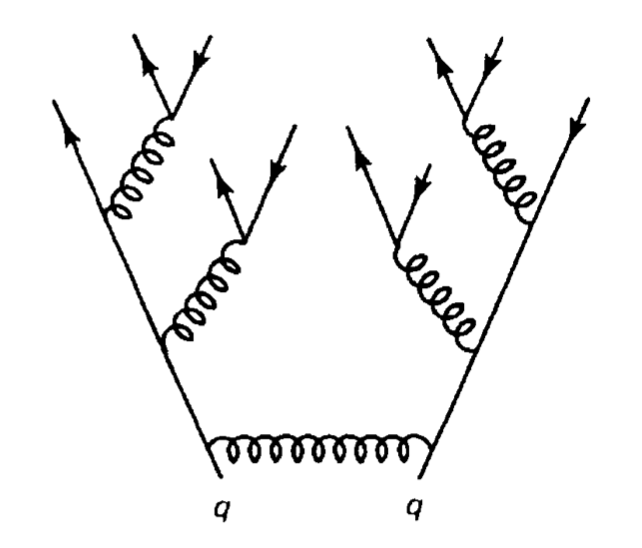
\includegraphics[width=0.5\textwidth]{figures/ch1/jet_feynmann.png}
	\caption{An example Feynmann diagram of jet production}
	\label{fig:jet_feynmann}
\end{figure}

\section{Symmetries}

The Standard Model is a renormalizable quantum field theory that obeys the local symmetry $G_{SM}$:

\begin{equation}
	G_{SM} = SU(3)_C \cross SU(2)_L \cross U(1)_Y .
\end{equation}

The $SU(3)_C$ symmetry component represents the non-Abelian gauge group of QCD. There are 8 generators for the $SU_C (3)$ group which correspond to 8 types of gluon, each representing a different superposition of color charge \cite{pdg}. The $SU(2)_L \cross U(1)_Y$ symmetry group represents the electroweak sector of the Standard Model, which can be spontaneously broken into the electromagnetic and weak sectors. There are 4 generators for this group, which correspond to four massless gauge bosons $W^1$, $W^2$, $W^3$, and B. From these massless gauge bosons are formed the massive mediators of the weak force, the $W^-$, $W^+$ and $Z^0$ bosons, and the massless electromagnetic force carrier, the photon $\gamma$. Spontaneous symmetry breaking and the process by which gauge bosons acquire mass will be addressed in section \ref{sec:sponsymbrk}. \par

Noether's theorem \cite{Noether} stipulates that any continuous symmetry is associated with a conserved quantity. In the Standard Model, this means that the $SU(3)_C$ symmetry gives rise to conservation of color charge. The $SU(2)_L \cross U(1)_Y$ symmetry gives rise to conservation of electromagnetic charge. Conservation of spin results from the Poincar\'e symmetry described by the theory of special relativity, which combined with Noether's theorem gives us the conservation of energy, momentum, and angular momentum.\par

The SM Lagrangian is invariant under $CPT$ symmetry, or charge, parity, and time reversal. Charge conjugation ($C$) transform a particle into its corresponding antipaticle by reversing the charge and other quantum numbers. Parity conjugation ($P$) reverses spatial coordinates, which transforms left-handed particles into right-handed particles and vice-versa. Time reversal ($T$) is the theoretical process of reversing time. The $L$ subscript in the $SU(2)_L$ group indicates that this symmetry only applies to left-handed fermions. As a result, the $W^{1,2,3}$ gauge bosons of $SU(2)_L$ only interact with left handed particles, a process which maximally violates P-symmetry in the weak force. A small amount of the CP symmetry violation is also observed in the Standard Model, through the decays of strange flavored mesons~\cite{strange_mesons} and $b$-mesons~\cite{bmeson}. The CPT theorem posits that the violation of CP symmetry implies that T-symmetry must also be violated, so that CPT is a preserved symmetry.\par

\subsection{Spontaneous Symmetry Breaking and The Higgs Mechanism}
\label{sec:sponsymbrk}

Spontaneous symmetry breaking is the process by which a Lagranian obeys a symmetry at high energies, but exhibits asymmetric behavior at lower energies. The electroweak symmetry group is spontaneously broken as $SU(2)_L \cross U(1)_Y \rightarrow U(1)_{EM}$. The quantity conserved by the $SU(2)_L$ symmetry is weak isospin $T_{1,2,3}$, while the quantity conserved by $U(1)_Y$ symmetry is weak hypercharge $Y$. Below very high energies, the presence of the Higgs field causes the electroweak symmetry to break. The Higgs field is a scalar field which forms a complex doublet of the $SU(2)$ symmetry group, with four degrees of freedom. The shape of the Higgs field potential, shown in Figure \ref{fig:higgs_field}, results in a ground state with a non-zero vacuum expectation value; thus the Higgs field takes a non-zero value throughout all space, which breaks the symmetry of the weak isopsin $SU(2)$ group. \par

\begin{figure}
	\centering
	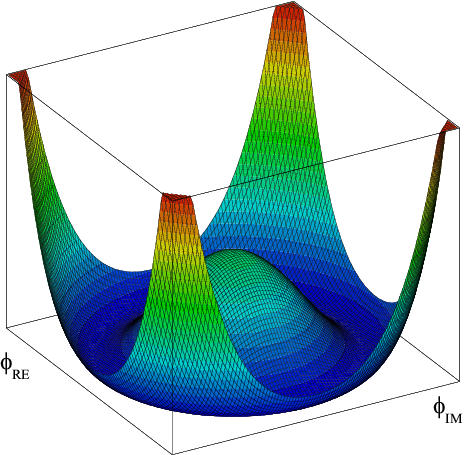
\includegraphics[width=0.3\textwidth]{figures/ch1/higgs_field.png}
	\caption{An illustration of the ``hat shaped" potential of the Higgs field, resulting in a non-zero vacuum expectation value. }
	\label{fig:higgs_field}
\end{figure}

The interaction with the Higgs field mixes the four massless gauge bosons $W^{1,2,3}$ and $B$. Three Higgs field degrees of freedom mix with the massless gauge bosons, resulting in three massive gauge bosons $W^-$, $W^+$ and $Z^0$. The massless photon $\gamma$ is created from the components of the massless gauge bosons which do not interact with the Higgs field. The scalar Higgs boson arises from the one unmixed degree of freedom the Higgs field. Spontaneous symmetry breaking also violates the conservation of weak isospin and weak hypercharge, leaving only electromagnetic charge ($Q = T_3 + \frac{1}{2}Y$) as a conserved quantity associated with the $U(1)_{EM}$ symmetry. 

\section{Experimental Validation of the Standard Model}

The theoretical framework of the Standard Model coalesced into a unified theory in the mid-20th century. A cascade of discoveries providing empirical evidence for the model followed closely. In the 1960s, three quarks (up, down and strange) and four leptons (electron, muon, and their associated neutrinos) were the known particulate building blocks of matter and the Standard Model. The discovery of the charm quark in 1974, through the observation of the $J/\psi$ meson \cite{SLAC_J}\cite{BNL_J}, confirmed the existence of a fourth quark flavor. The discovery of the $\tau$ in 1975 \cite{tau} provided the first evidence of a 3rd generation of matter. This was quickly followed by the observation of the $\Upsilon$ meson in 1977 \cite{upsilon}, which provided evidence for the existence of a fifth quark, the $b$ quark (bottom, or beauty). The existence of a 3rd generation of fermion also explained the observation of CP violation in the weak force, as it allowed for the addition of a complex phase in the CKM matrix (a unitary matrix which describes flavor mixing in the weak interaction). The top quark ($t$) and tau neutrino ($\nu_\tau$) were predicted at this point as the final building blocks of three complete generations of fermions, and they were discovered by experimental observation around the turn of the 21st century \cite{top_CDF} \cite{top_D0} \cite{tau_nu}. \par

The W and Z bosons were predicted by the Standard Model, but to observe them required the construction of a particle accelerator powerful enough to produce them. They were finally observed at CERN in 1983 by the UA1 and UA2 experiments \cite{UA1} \cite{UA2} at the newly constructed Super Proton Synchrotron (SPS). Their masses were observed to be compatible with the masses predicted by the Standard Model nearly a decade earlier. The final missing piece then was confirming the existence of the Higgs, which again required the construction of a newer and more powerful collider. CERN achieved this with the construction of the Large Hadron Collider (LHC), and in 2012 the ATLAS and CMS experiments announced the discovery of the Higgs particle \cite{higgs_CMS} \cite{higgs_ATLAS}. 

\section{Limitations of the Standard Model}
\label{sec:lim_sm}

While the Standard Model has enjoyed decades of experimental results which confirm its predictions, there are several glaring shortcomings. The observed phenomenon for which the Standard Model provides no explanation are summarized below.

\begin{itemize}
  \item Gravity - the Standard Model does not account for the fourth fundamental force of gravity.
  \item Dark Matter - there is no viable candidate to explain the existence of dark matter, a non-interacting form of matter which must exist to account for gravitational observations which cannot be explained by general relativity, such as the motion of galaxies, gravitational lensing, and the structure of the universe \cite{dm}.
  \item Matter-Antimatter asymmetry - the level of CP violation in the Standard Model isn't sufficient to explain the large discrepancy between the amount of matter and the amount of antimatter in the universe today, and the origins of this imbalance are not understood.
  \item Neutrino masses - the Standard Model assumes that neutrinos are massless and provides no mechanism for them to acquire mass. However, observations of neutrino oscillations indicates they posses some small non-zero mass \cite{neutrino_osc}.
\end{itemize}

In addition to these unexplained natural phenomenon, there are several questions about the \textit{naturalness} of the Standard Model. The principle of naturalness states that dimensionless ratios between physical constants should be of order 1, and that nature should not be arbitrarily fine-tuned. While this is largely an aesthetic argument, it points to many aspects of the Standard Model for which there exists no natural explanation.

\begin{itemize}
  \item Strong CP - while CP symmetry is violated in the weak force, observations indicate that it is preserved by the strong force \cite{strongCP}. The Standard Model predicts that CP violation in the strong force is possible. There is no principle which motivates this incongruity between the weak force and strong force.
  \item Hierarchy Problem - The wide range of masses for elementary particles and the wide range of scales at which the four fundamental forces operate is not motivated by the SM. Specifically, it is not understood why the Higgs mass is observed to be well below the Plank scale $\lambda$, which is the energy level at which the effects of quantum gravity become significant. QFT indicates that the Higgs mass is determined by contributions from all energy scales including $\lambda$, meaning that its observed mass is inexplicably small.
\end{itemize}

The limitations of the Standard Model provide a road map for theoretical and experimental particle physicists, who seek to develop new theories which account for these observations, and then to find evidence which might support these \textit{Beyond the Standard Model} (BSM) theories. The next chapter will introduce the BSM theories which motivate the physics search presented in this thesis. 
  
